\documentclass{beamer}
\usepackage{tikz}
\usetikzlibrary{shapes}
\usepackage[utf8]{inputenc}
\usetheme{Boadilla}
\usecolortheme{seahorse}
\usepackage{epstopdf}
\usepackage{subfig}


\author[F.Paterno] {\textbf {Fabio Paterno} \\ \footnotesize Presented By \\ Ashiqur Rahman (1605103) \\Md. Zunaed Karim (1605113) \\ Tasin Ishmam (1605115)}
\title[A Theory of User-interaction Objects
]{A Theory of User-interaction Objects}
\institute[CNUCE]{Centro Nazionale Universitario di Calcolo Elettronico, Institute of CNR}
\date{}


\tikzstyle{oval} = [ellipse,draw,text centered]
\tikzstyle{circ} = [circle,draw,text centered]
\tikzstyle{rec} = [rectangle,draw,text centered]
\tikzstyle{dia} = [diamond,aspect=4,draw]
\tikzstyle{para} = [trapezium, trapezium left angle=70, trapezium right angle=110,draw]


\begin{document}
	\frame{\titlepage}
	\begin{frame}
		\tableofcontents
	\end{frame}
	
	
	\section{Motivation}
	\begin{frame}
		\frametitle{User Experience}
		User Interfaces are a important part of the user experience. \\
		They directly
		 affect the users ability to analyze and understand the information presented. \newline 
		
		
\pause
\begin{figure}
	\centering
	\subfloat[Fiverr Website\label{fig:a}]{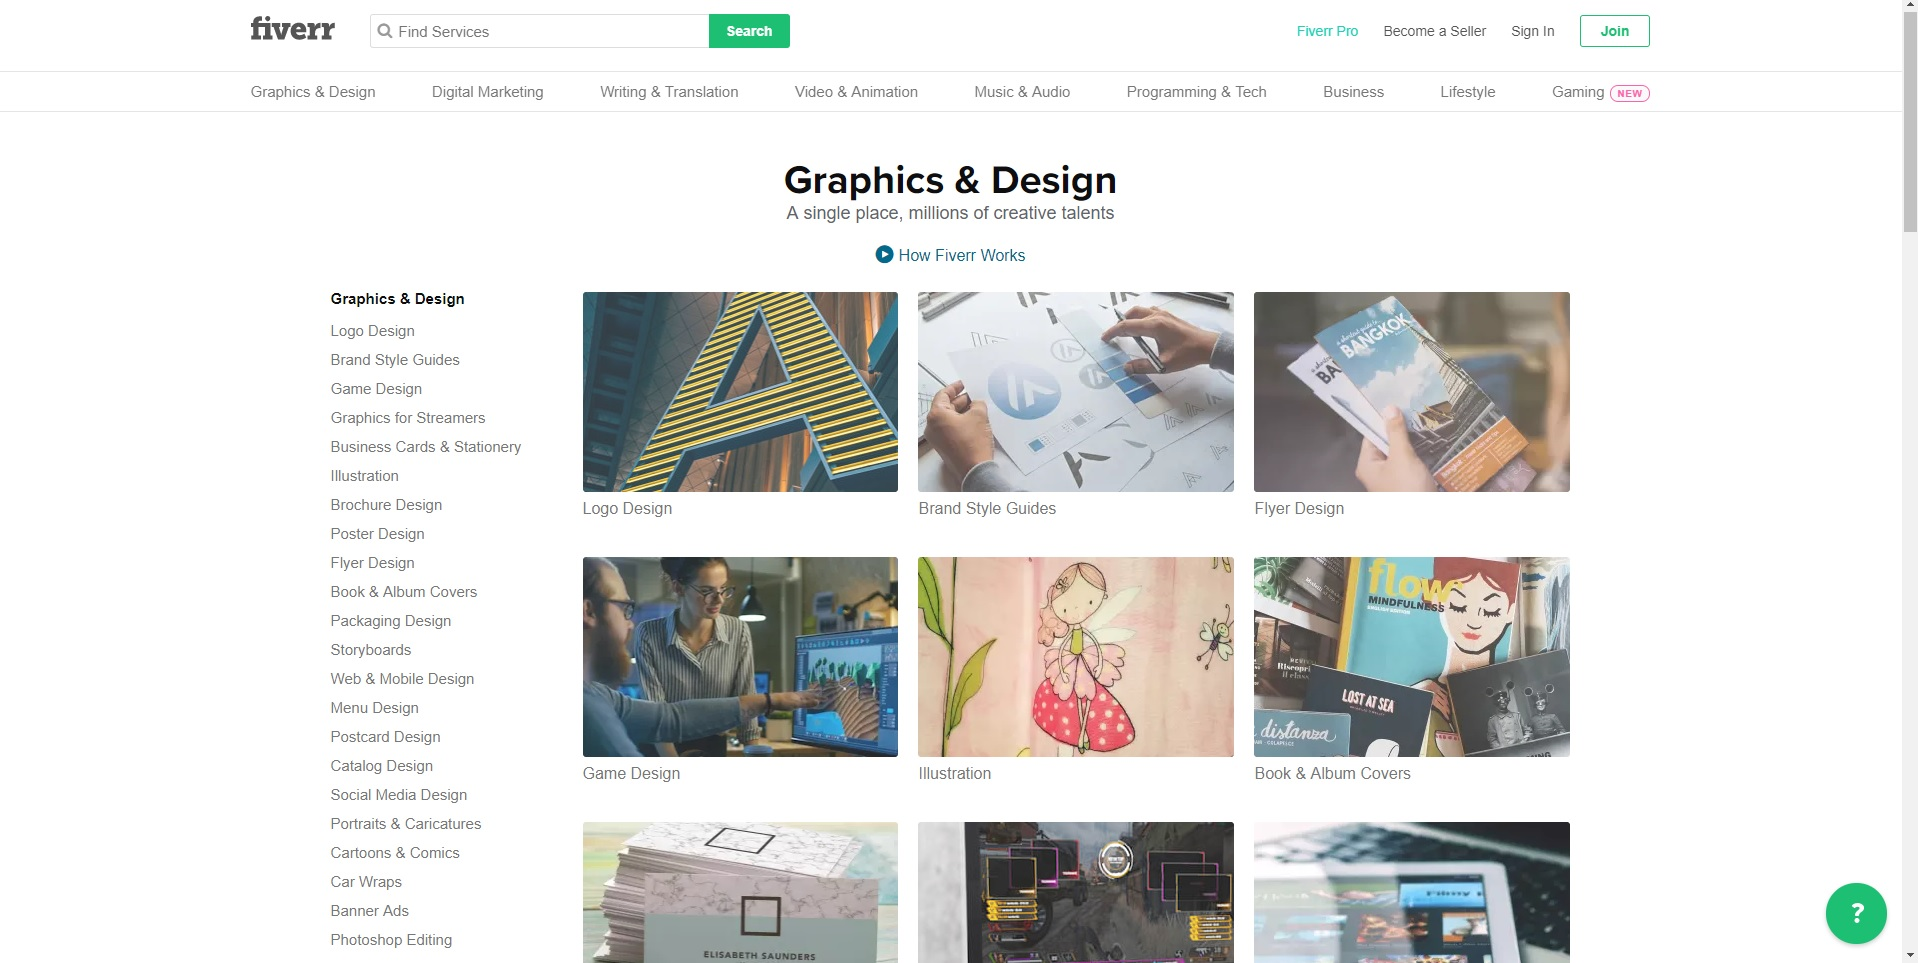
\includegraphics[scale=0.083]{fiver.eps}}\qquad
	\subfloat[Craigslist Website\label{fig:b}]{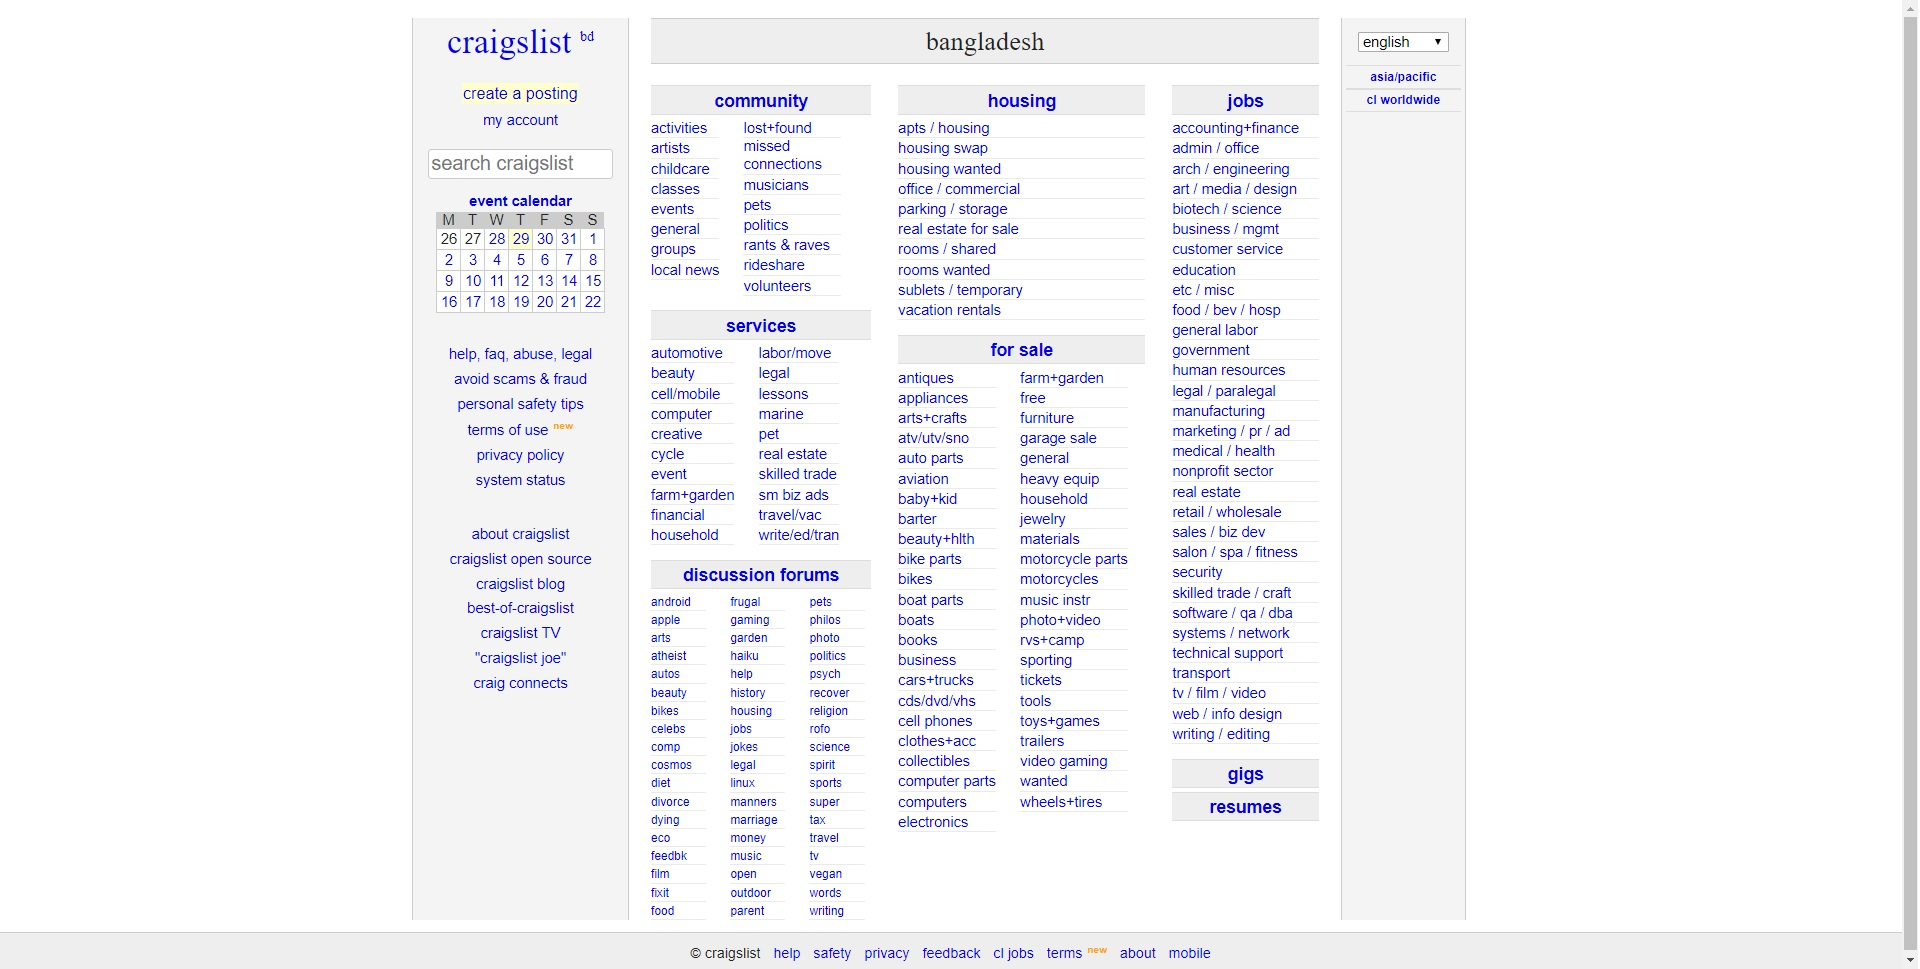
\includegraphics[scale=0.083]{craigslist.eps}}
	\caption{Good vs Bad UI}
\end{figure}
		
	\end{frame}
	
	\begin{frame}
		\frametitle{Motivation}
		Taking a mathematical approach to UI design helps us: \\
		\begin{itemize}
			\item Provide useful indicators and guidelines to UI designers during design refinement phase\pause
			\item Create better automated tools for UI design and testing \\ (Around 80\% software companies use such tools for testing their UI \footnote{The 2018 State of Testing Report - Smartbear})\pause
			\item Create more reusable UI elements
		\end{itemize}
	\end{frame}
	
	\section{Problem Definition}
	\begin{frame}
		\frametitle{Problem Definition}	
		How to define user interface systems so that  
		\begin{itemize}
			\item They can be described formally using precise mathematical notation 
			\pause
			\item Their behavior and properties can be methodically evaluated
		\end{itemize}
		
	\end{frame}
	
	
	
	
	
	\section{Previous Works}
	\begin{frame}
		\frametitle{Previous Works}
		\addtobeamertemplate{block end}{}{\vspace*{1cm}}
		
			\begin{block}{M. Harrison \& H. Thimbleby (1990), \textit{Cambridge University Press}}
			Formal Methods in Human-Computer interaction
		\end{block}
	\pause
		\begin{block}{B. A. Myers, \textit{ACM Transactions on Information Systems 8}}
			A new Model for handing input
		\end{block}
		\pause
		\begin{block}{L. Cinque et al. (1990), \textit{Proceedings of IEEE Workshop on Visual Languages}}
			Towards a formal specification methodology for iconic interface design
		\end{block}
	\end{frame}


%PART - 2 
%\section{What is a UIS?}
%\begin{frame}{What is a UIS?}
 %  	Every Application has 3 major components.
  % 	\begin{figure}[h]
   % 	\centering
    %	\begin{tikzpicture}
    %	\node[rec,xshift=-1cm](Application) {Application};
    %	\node[rec,right of=Application,xshift=2cm](UIS) {UIS};
    %	\node[rec,right of=UIS,xshift=2cm](User) {User};\pause
    %	
    %	\draw[->] (Application.north) -- ++(0,2) -| (UIS);
    %	\draw[->] (UIS.south) -- ++(0,-2) -| (User);
    %	\draw[->] (User) -- (UIS);
   % 	\draw[->] (UIS) -- (Application);
    	  	
  %  	\end{tikzpicture}
 %   \end{figure}
%\end{frame}

\section{Building Block of a UIS}
\begin{frame}{Building Block of a UIS : Interactor}
	As we can see UIS is the component that communicates between the user end and the application end.Each UIS is basically a composition of a much smaller components.\\
	 And we are calling it the \textbf{'Interactor'}   
\end{frame}

\section{Architectural Model of an Interactor}
\begin{frame}{Architectural Model of an Interactor}
	An Interactor consists of 4 architectural components.
	\begin{itemize}
		\item Measure
		\item Control
		\item Collection
		\item Presentation 
	\end{itemize}
\end{frame}
\begin{frame}
	\begin{figure}[h]
		\centering
		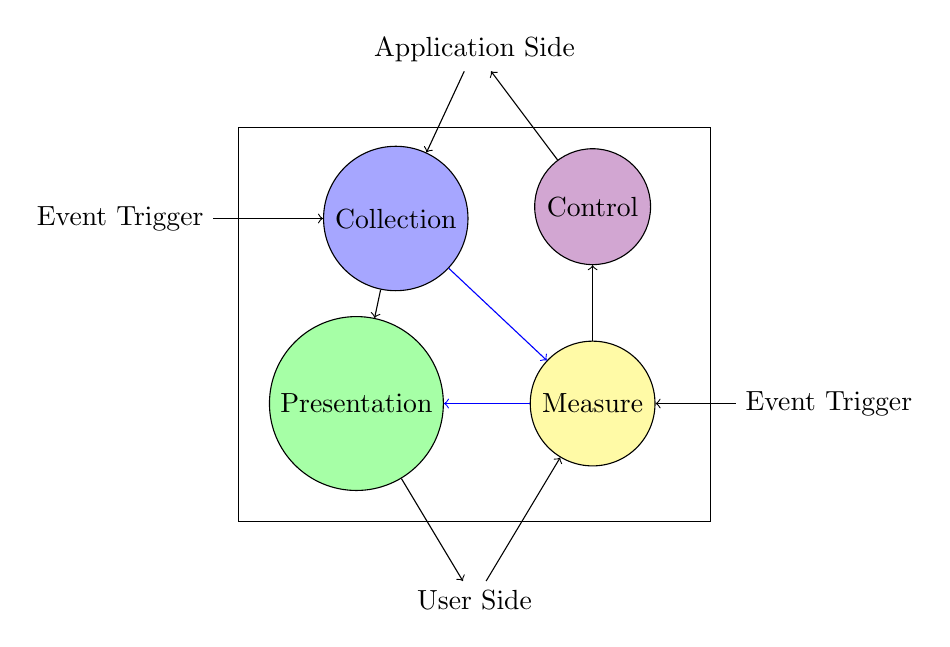
\begin{tikzpicture}
		
		\node[rec,minimum width = 6cm,minimum height = 5cm,xshift = 0.5cm]() {};
		\node[circ,fill=blue!35,xshift=-0.5cm,yshift = 1.35cm](Collection) {Collection};
		\node[circ,fill=green!35,xshift=-1cm,yshift=-1cm](Presentation) {Presentation};
		\node[circ,fill=yellow!35,xshift=2cm,yshift=-1cm](Measure) {Measure};
		\node[circ,fill=violet!35,xshift=2cm,yshift=1.5cm](Control) {Control};
		\node[yshift=3.5cm,xshift=0.5cm](Application) {Application Side};
		\node[yshift=-3.5cm,xshift=0.5cm](User) {User Side};\pause
		
		\draw[->] (User) -- (Measure); \pause
		\node[xshift=5cm,yshift=-1cm](TriggerUser) {Event Trigger};
		\draw[->] (TriggerUser) -- (Measure);\pause
		\draw[->] (Measure) -- (Control); 
		\draw[->,blue] (Measure) -- (Presentation);\pause
		\draw[->] (Control) -- (Application);\pause
		
		\draw[->] (Application) -- (Collection);\pause
		\node[xshift=-4cm,yshift=1.35cm](TriggerApp) {Event Trigger};
		\draw[->] (TriggerApp) -- (Collection);\pause
		\draw[->] (Collection) -- (Presentation);
		\draw[->,blue] (Collection) -- (Measure);\pause
		
		\draw[->] (Presentation) -- (User);
				
		\end{tikzpicture}
	\end{figure}
	
\end{frame}

\section{How It Works?}
\begin{frame}{How It Works}
Interactor performs two functions to the data.
\begin{itemize}
	\item Input Function also called, Internal Behaviour
	\item Output Function also called, External Behaviour
\end{itemize}
\end{frame}
\begin{frame}
\begin{figure}[h]
	\centering
	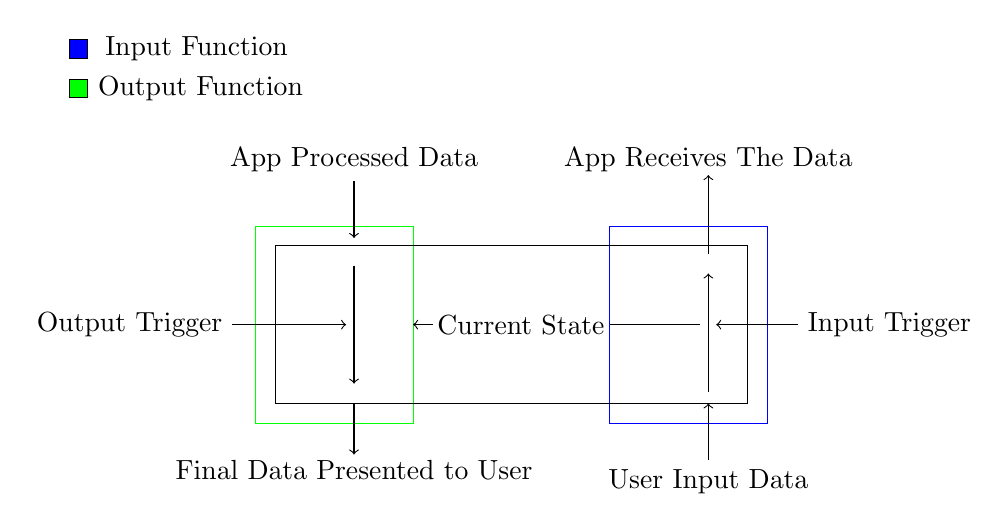
\begin{tikzpicture}
	%\node[yshift=3cm](Application) {Application Side};
	%\node[yshift=-2cm](User) {User Side};
	\node[rec,fill=blue,xshift=-5.5cm,yshift=4cm](inputFunc){};
	\node[right of=inputFunc,xshift=0.5cm](){Input Function};
	\node[rec,blue,minimum width = 2cm,minimum height = 2.5cm,xshift = 2.25cm,yshift=0.5cm](){};
	
	\node[rec,fill=green,below of=inputFunc,yshift=0.5cm](outputFunc){};
	\node[right of=outputFunc,xshift=0.55cm](){Output Function};
	\node[rec,green,minimum width = 2cm,minimum height = 2.5cm,xshift = -2.25cm,yshift=0.5cm](){};
	
	\node[rec,minimum width = 6cm,minimum height = 2cm,yshift=0.5cm]() {};\pause
	
	\node[xshift=2.5cm,yshift=-1.5cm](Im) {User Input Data};
	\draw[->] (Im) -- ++ (0,1);\pause	
	\node[xshift=4.8cm,yshift=0.5cm](Bool1) {Input Trigger};
	\draw[->] (Bool1) -- (2.6,0.5);\pause
	\draw[->] (2.5,-0.35) -- ++ (0,1.5);
	\draw[->] (2.5,1.4) -- ++ (0,1);
	\node[xshift=2.5cm,yshift=2.6cm](Inp) {App Receives The Data};\pause
	\draw[-] (2.4,0.5) --  (1.25,0.5);
	\node[xshift=0.12cm,yshift=0.5cm]{Current State};
	\draw[->] (-1.0,0.5) --  (-1.25,0.5);\pause
	
	
	
	% end of input behaviour
	
	
	\node[xshift=-2cm,yshift=2.6cm](Ic) {App Processed Data};
	\draw[->] (Ic) -- ++ (0,-1);\pause
	\node[xshift=-4.85cm,yshift=0.5cm](Bool2) {Output Trigger};
	\draw[->] (Bool2) -- (-2.1,0.5);\pause
	\draw[->] (-2,-0.5) -- ++ (0,-0.65);
	\draw[->] (-2,1.25) -- ++ (0,-1.5);	
	
	\node[xshift=-2cm,yshift=-1.35cm](Out) {Final Data Presented to User};
	
	
	
	
	\end{tikzpicture}

\end{figure}

\end{frame}


\section{Formal Definition of an Interactor and UIS}
\begin{frame}{Definition of an Interactor}
	
	Now, we can finally define an Interactor mathematically.
	\begin{block}{An Interactor is a pair of functions}
		$$ I = (FI,FO) $$
	\end{block}
	
	Where,\\
	
	 FI = Input Function 
	 FO = Output Function 
	
	
\end{frame}




	\section{Properties of UIS}
	
	\begin{frame}{Definition of an UIS}
	So, We can define an UIS as,
		
		\begin{block}{An UIS is a composition of of Interactors}
			$$ UIS =  \{I1,I2,I3,I4,........\}  $$
		\end{block}

		\begin{block}{Equivalence Property}
		We call 2 UIS equivalent if for every possible input, they produce the same result
		\end{block}
	 
	\end{frame}
   	
	\begin{frame}{Properties of UIS Using Graphs}   	
	\begin{figure}[h]
    	\centering
    	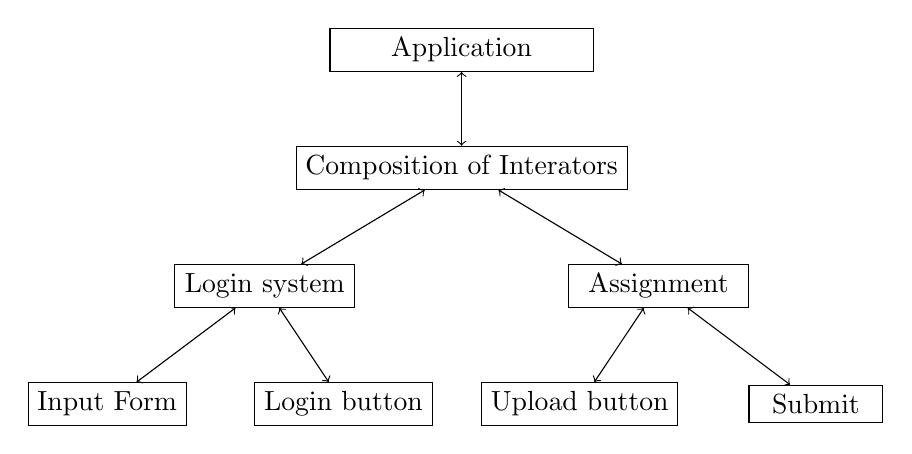
\begin{tikzpicture}
    	
    	\node[rec,minimum width={width("Magnetometeraaaaaa")+2pt}](application) {Application};
    	\node[rec,yshift=-0.5cm,minimum width={width("Magnetometeraaaaaa")+2pt},below of=application](composition) {Composition of Interators};
    	\node[rec,xshift=-2.5cm,yshift=-0.5cm,minimum width={width("Magnetometer")+2pt},below of=composition](login) {Login system};
    	\node[rec,xshift=-2cm,yshift=-0.5cm,minimum width={width("Magnetom")+2pt},below of=login](form) {Input Form};
    	\node[rec,xshift=2cm,minimum width={width("Magnetom")+2pt},right of=form](button) {Login button};
    	\node[rec,xshift=4cm,minimum width={width("Magnetometer")+2pt},right of=login](assignment) {Assignment};
    	\node[rec,xshift=2cm,minimum width={width("Magnetom")+2pt},right of=button](upload) {Upload button};
    	\node[rec,xshift=2cm,minimum width={width("Magnetom")+2pt},right of=upload](submit) {Submit};
		\pause

		\draw[<->] (composition) -- (application);
    	\draw[<->] (login) -- (composition);
    	\draw[<->] (form) -- (login);
    	\draw[<->] (button) -- (login);
    	\draw[<->] (assignment) -- (composition);
    	\draw[<->] (upload) -- (assignment);
    	\draw[<->] (submit) -- (assignment);
    	\end{tikzpicture}
    \end{figure}
   	
   	\end{frame}
   	
   	
	\begin{frame}{Communication Consistency}   	
	\begin{figure}[h]
    	\centering
    	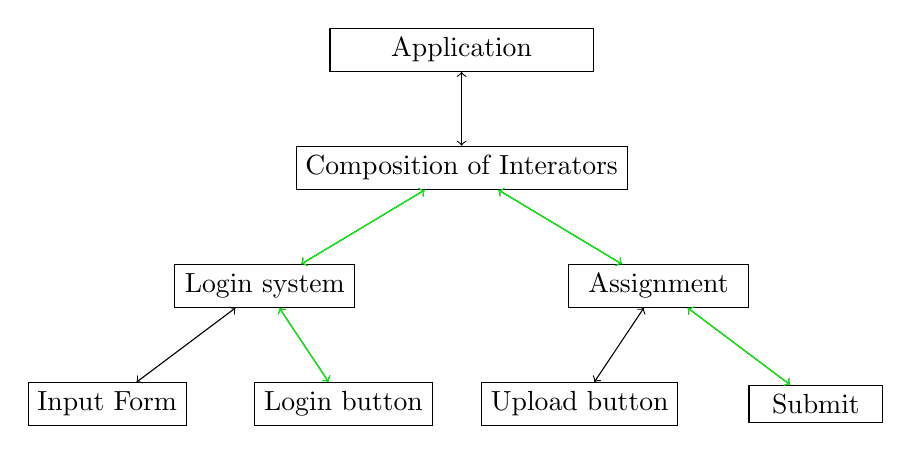
\begin{tikzpicture}
    	
    	\node[rec,minimum width={width("Magnetometeraaaaaa")+2pt}](application) {Application};
    	\node[rec,yshift=-0.5cm,minimum width={width("Magnetometeraaaaaa")+2pt},below of=application](composition) {Composition of Interators};
    	\node[rec,xshift=-2.5cm,yshift=-0.5cm,minimum width={width("Magnetometer")+2pt},below of=composition](login) {Login system};
    	\node[rec,xshift=-2cm,yshift=-0.5cm,minimum width={width("Magnetom")+2pt},below of=login](form) {Input Form};
    	\node[rec,xshift=2cm,minimum width={width("Magnetom")+2pt},right of=form](button) {Login button};
    	\node[rec,xshift=4cm,minimum width={width("Magnetometer")+2pt},right of=login](assignment) {Assignment};
    	\node[rec,xshift=2cm,minimum width={width("Magnetom")+2pt},right of=button](upload) {Upload button};
    	\node[rec,xshift=2cm,minimum width={width("Magnetom")+2pt},right of=upload](submit) {Submit};

		\draw[<->] (composition) -- (application);
    	\draw[<->] (login) -- (composition);
    	\draw[<->] (form) -- (login);
    	\draw[<->] (button) -- (login);
    	\draw[<->] (assignment) -- (composition);
    	\draw[<->] (upload) -- (assignment);
    	\draw[<->] (submit) -- (assignment);
    	
    	\filldraw[green,<->] (submit) -- (assignment);
    	\filldraw[green,<->] (assignment) -- (composition);
		\filldraw[green,<->] (login) -- (composition);
    	\filldraw[green,<->] (button) -- (login);
    	  	
    	\end{tikzpicture}
    \end{figure}
    
    \begin{block}{Communication Consistency}
			The UIS should have at least one path.
	\end{block}
   	
   	\end{frame}
   	
   	
	\begin{frame}{Connectivity Property}   	
	\begin{figure}[h]
    	\centering
    	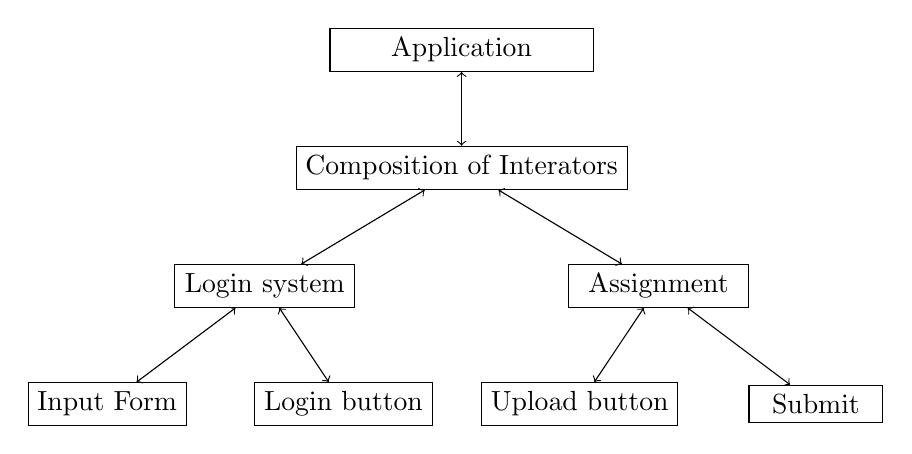
\begin{tikzpicture}
    	
    	\node[rec,minimum width={width("Magnetometeraaaaaa")+2pt}](application) {Application};
    	\node[rec,yshift=-0.5cm,minimum width={width("Magnetometeraaaaaa")+2pt},below of=application](composition) {Composition of Interators};
    	\node[rec,xshift=-2.5cm,yshift=-0.5cm,minimum width={width("Magnetometer")+2pt},below of=composition](login) {Login system};
    	\node[rec,xshift=-2cm,yshift=-0.5cm,minimum width={width("Magnetom")+2pt},below of=login](form) {Input Form};
    	\node[rec,xshift=2cm,minimum width={width("Magnetom")+2pt},right of=form](button) {Login button};
    	\node[rec,xshift=4cm,minimum width={width("Magnetometer")+2pt},right of=login](assignment) {Assignment};
    	\node[rec,xshift=2cm,minimum width={width("Magnetom")+2pt},right of=button](upload) {Upload button};
    	\node[rec,xshift=2cm,minimum width={width("Magnetom")+2pt},right of=upload](submit) {Submit};

		\draw[<->] (composition) -- (application);
    	\draw[<->] (login) -- (composition);
    	\draw[<->] (form) -- (login);
    	\draw[<->] (button) -- (login);
    	\draw[<->] (assignment) -- (composition);
    	\draw[<->] (upload) -- (assignment);
    	\draw[<->] (submit) -- (assignment);
    	  	
    	\end{tikzpicture}
    \end{figure}
  
    \begin{block}{Connectivity Property}
			Every component should be connected with one another.
	\end{block}
   	
   	\end{frame}
	
	\section{Benifit of Having a Precise Model}
	\begin{frame}{Benifit of Having a Precise Model}
		We can also use these properties to
	    \begin{itemize}
	    	\item Develop a precise model to identify redundancy and common mistakes in UIS design\pause
	    	\item Develop reusable libraries for UI design\pause
	    	\item Build automated tools for building and fixing UI
	    \end{itemize}
	\end{frame}
	
	\begin{frame}
		\begin{center}
			\Huge Thank You!
		\end{center}
	\end{frame}

\end{document}